%----------------------------------------------------------------------------
\chapter{序論}
\label{sec:josho}
%----------------------------------------------------------------------------

フランスとスイスの国境にある欧州原子力研究機構 (CERN) に設置されている大型陽子衝突型加速器 (LHC) では、現在、素粒子物理学の基礎となっている標準模型の精密測定や標準模型を超える物理現象の探索が行われている。 ATLAS実験は HC上にある4つの衝突点の1つで行われている実験であり、ATLAS 検出器を用いて 生成粒子の測定が行われている。LHCでは加速器のアップグレード(HL-LHC)を予定しており、これに向けてATLAS検出器のアップグレードを行う。この章ではLHC-ATLAS実験とそのアップグレード計画について説明する。



%----------------------------------------------------------------------------
\section{素粒子標準模型}
\label{sec:}
%----------------------------------------------------------------------------
ganbatte kakima shou !!




%----------------------------------------------------------------------------
\subsection{標準模型の概要}
\label{sec:}
%----------------------------------------------------------------------------





%----------------------------------------------------------------------------
\subsection{標準模型を超えた新物理の探索}
\label{sec:}
%----------------------------------------------------------------------------





%----------------------------------------------------------------------------
\section{LHC}
\label{sec:LHC}
%----------------------------------------------------------------------------

\begin{figure}[tbp]
  \centering
  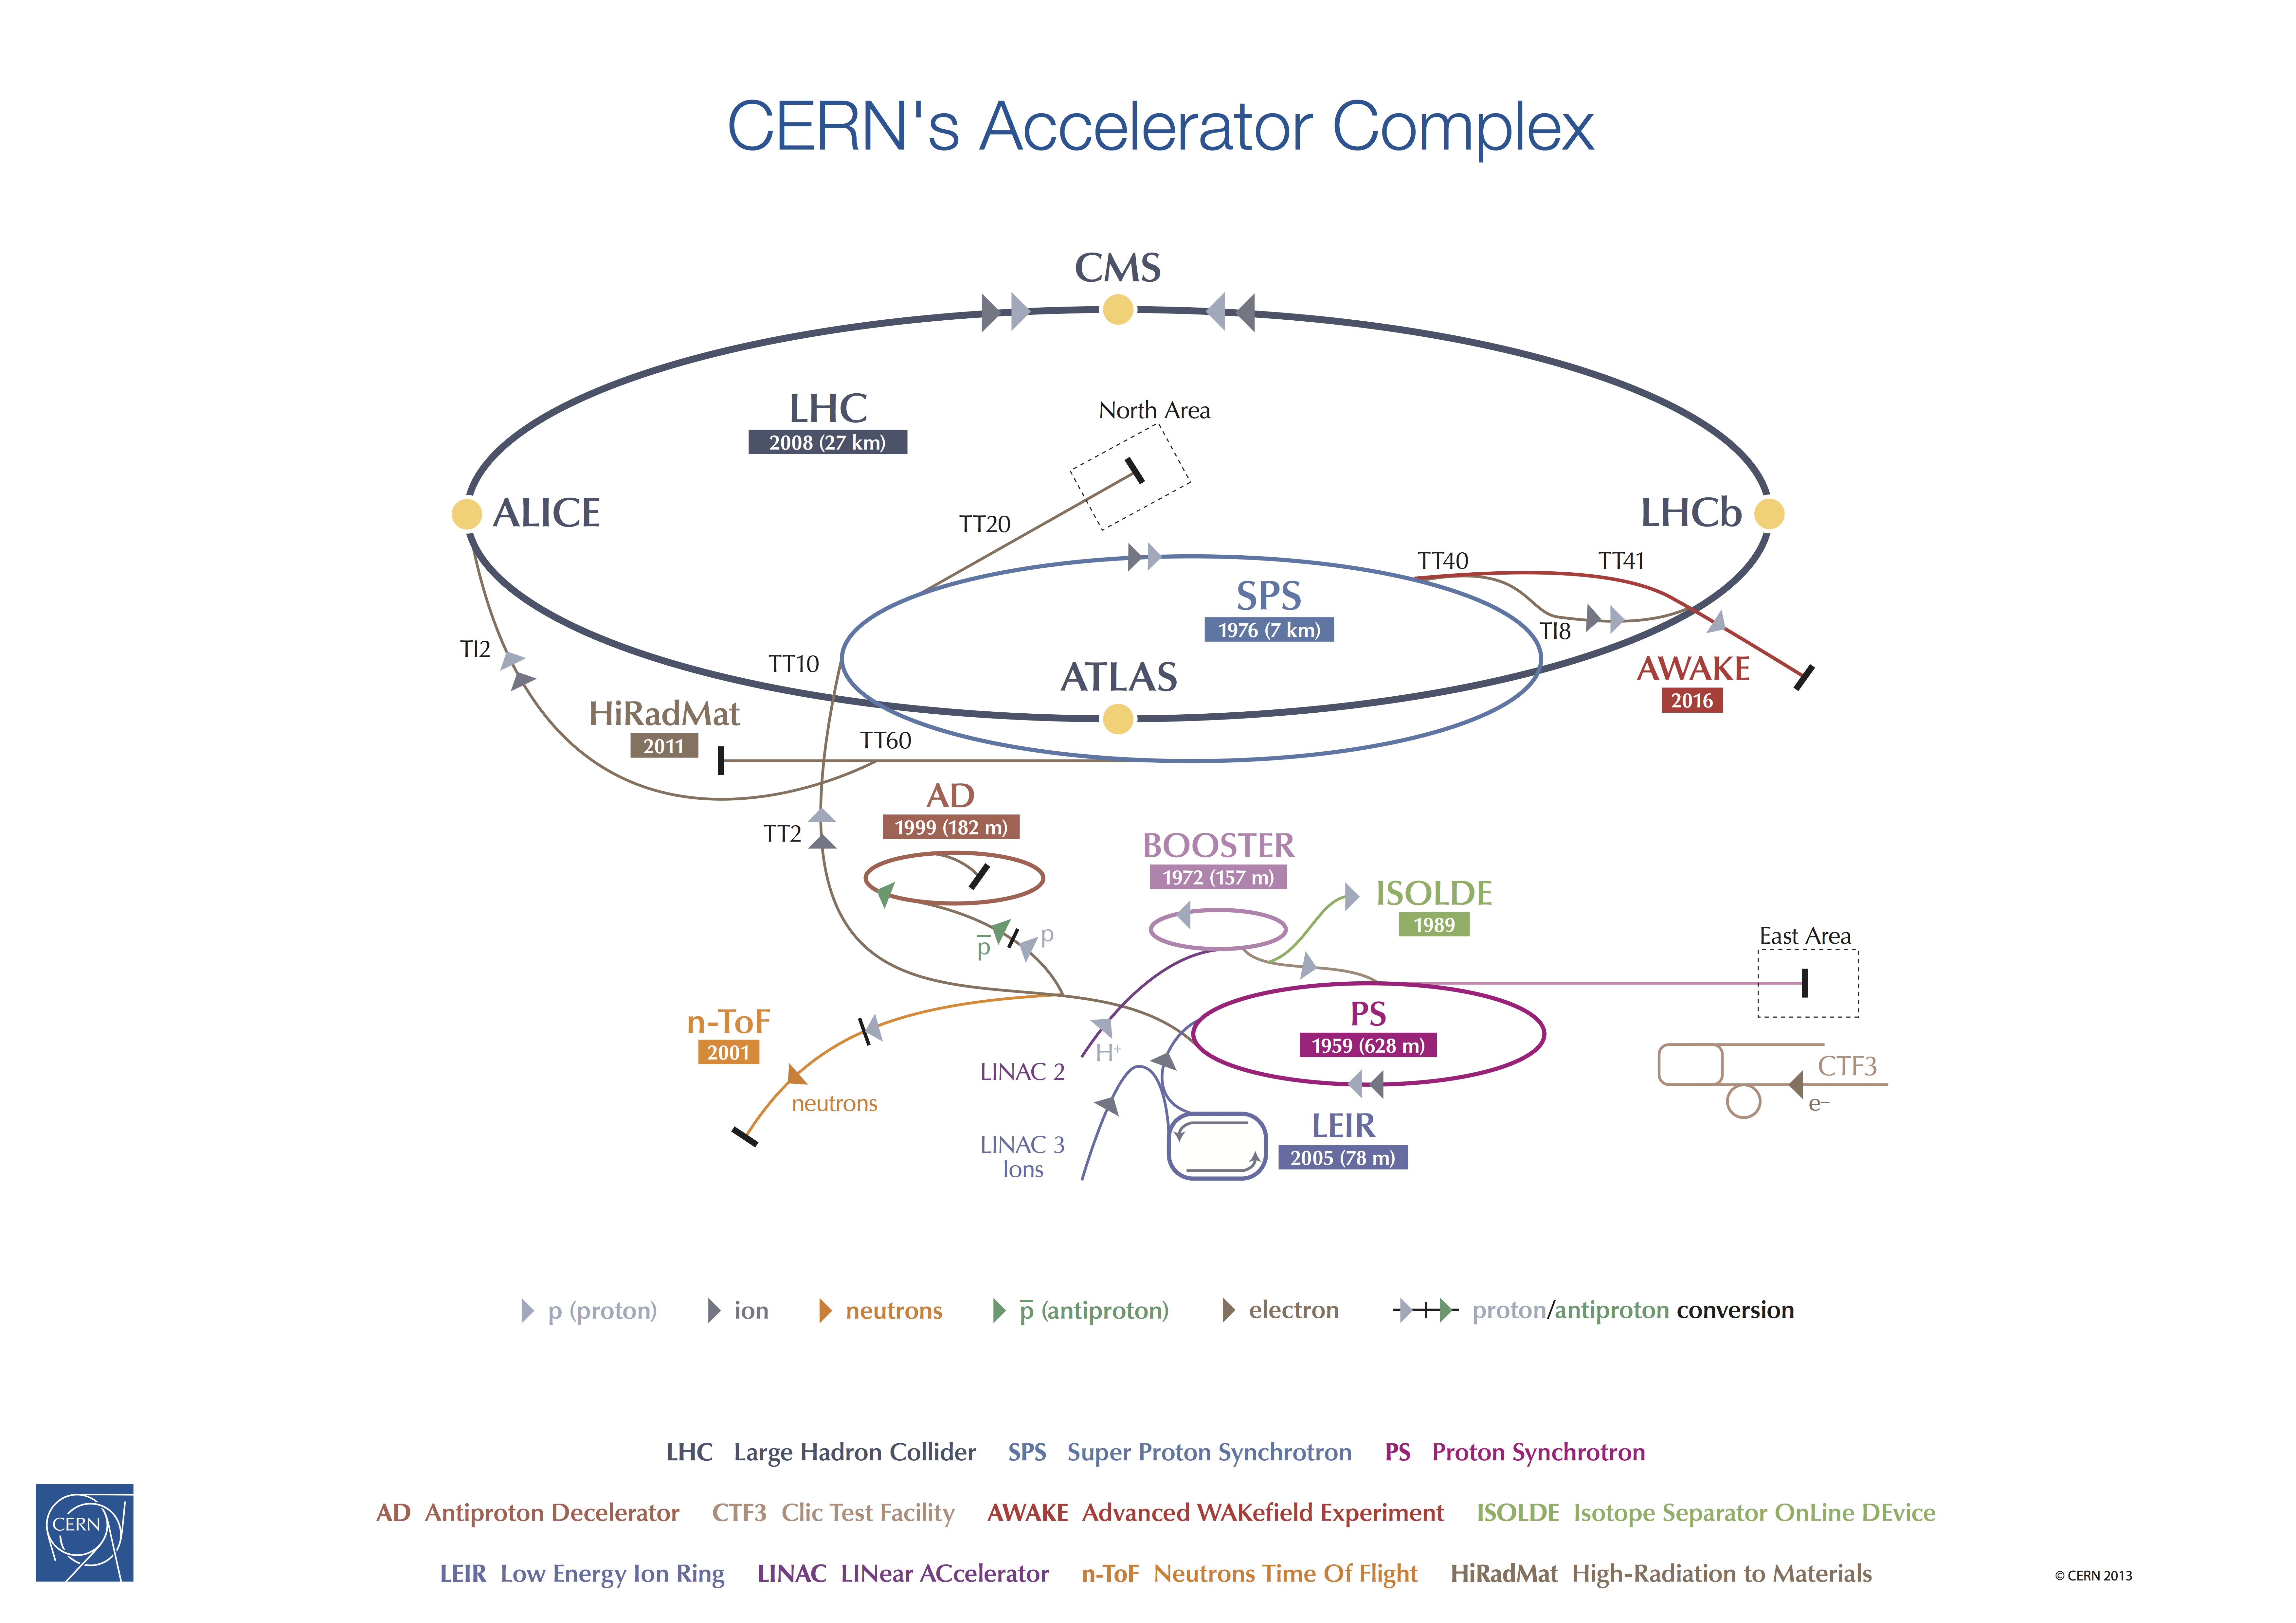
\includegraphics[height=8cm,keepaspectratio]{LHC.jpg}
  \caption[ATLAS検出器]{LHCの全体図 \cite{LHC} }
  \label{fig:LHC}
\end{figure}


LHC(\textbf{L}arge \textbf{H}adron \textbf{C}ollider)は欧州原子核研究機構(CERN)に建設された、周長がおよそ27\ \si{km}の陽子・陽子衝突型加速器である。陽子ビームの重心系エネルギーは世界最高のエネルギーである14\ \si{TeV}に到達できるよう設計されている。この世界最高のエネルギーを用いて、標準模型の精密測定やそれを超える新物理の探索がLHCの主な目的である。

\subsection{LHCの基本構造}
\fref{fig:LHC}にCERNに設置されている加速器・検出器の全体図を示す。陽子を生成し、加速器によって段階的に加速された2本の陽子ビームが、LHC周上において衝突する。


金属製の円筒に水素ガスを注入し、電場を用いて水素分子を陽子と電子に分離する。LHCのビームは、最大2808個のバンチと呼ばれる陽子のかたまりから構成され、$1.15\times 10^{11}$個の陽子が1バンチとして加速される。すなわち、LHCにおいて陽子陽子衝突から物理現象の探索をするためには、$2\ \mathrm{beams} \times 2808\ \mathrm{bunches}\times 1.15\cdot10^{11}\approx 6\cdot 10^{14}$個の陽子を生成する必要がある。

生成された陽子バンチは、初めに線形加速器 (LINAC\ 2)によって$50\ \si{MeV}$まで加速される。その後、陽子シンクロトロンブースター(PBS)、陽子シンクロトロン加速器(PS)、スーパーシンクロトロン加速器(SPS)によって段階的に$450\ \si{GeV}$まで加速され、2本の逆向きに加速された陽子バンチがLHCに投入される。LHCに投入された陽子バンチは$6.5\ \si{GeV}$(2018 年時点)まで加速されて、各衝突点において2つの陽子バンチが約$25\ \si{ns}$の間隔で衝突する。

LHCのビームパイプ上には4つの衝突点が設けられており、それぞれの衝突点において\ ATLAS(\textbf{A} \textbf{T}roidala \textbf{L}HC \textbf{A}pparata\textbf{S})、CMS(\textbf{C}ompact \textbf{M}uon \textbf{S}olenoid)、ALICE(\textbf{A} \textbf{L}arge \textbf{I}on \textbf{C}ollider \textbf{E}xperiment)、LHCb実験が行われている。




%----------------------------------------------------------------------------
\subsection{ルミノシティ}
\label{sec:luminosity}
%----------------------------------------------------------------------------

陽子ビームの強度を表すパラメータとして瞬間ルミノシティ$L$が用いられる。反応断面積$\sigma$の物理イベントが、1秒あたりに生じるイベント数 N は\eref{eq:lumi}で与えられる。
\begin{align}
  \label{eq:lumi}
  L = \gamma_{r} \frac{N_{b}^{2} n_{b} f_{rev}}{4\pi \epsilon_{n} \beta^*}R
\end{align}
ここで、$N_{b}$は1バンチあたりに含まれる粒子数、$n_{b}$は1ビームに含まれるバンチ数、$f_{rev}$はビームの回転周波数、$\gamma_{r}$は陽子ビームのローレンツ因子、$\epsilon_{n}$はビーム軸に垂直な平面でのビームの広がり、$\beta^{*}$は衝突点における振幅の大きさである。$F$は幾何学的損失係数という、ビーム衝突が有限の角度で起きることによる係数であり、\eref{eq:kikaf}で表される。
\begin{equation}
  \label{eq:kikaf}
  F=\left( 1+\left( \frac{\theta_{c}\sigma_{z}}{2\sigma^{*}} \right)^2 \right)^{-1/2}
\end{equation}
ここで、$\theta_c$は衝突時ビーム交叉角、$\sigma_z$は衝突時におけるバンチ長の標準偏差、$\sigma^*$は衝突時におけるのバンチ幅の標準偏差である。

単位時間あたりに起こる物理事象の回数$N_\mathrm{event}$は、瞬間ルミノシティ$L$と反応断面積$\sigma$を用いて\eref{eq:hannnou}のように表すことができる。
\begin{equation}
  \label{eq:hannnou}
  N_\mathrm{event} = \int L\ dt\ \sigma
\end{equation}



%----------------------------------------------------------------------------
\section{ATLAS実験}
\label{sec:ATLAS}
%----------------------------------------------------------------------------
\begin{figure}[tbp]
  \centering
  \includegraphics[height=7cm,keepaspectratio]{ATLAS.jpg}
  \caption[ATLAS検出器]{ATLAS検出器の全体図 \cite{ATLAS} }
  \label{fig:ATLAS}
\end{figure}


ATLAS実験はLHCの衝突点の一つに設置されている汎用型の検出器である。\fref{fig:ATLAS} に示すように、ATLAS検出器は直径25\ \si{m}長さ44\ \si{m}の円筒型をした巨大な検出器である。その中心に陽子の衝突点があり、LHCによって加速された陽子ビームが円筒の中心軸を通過するような構造になっている。
陽子ビームの衝突点である円筒の中心の内側から順に、内部飛跡検出器、電磁カロリメータ、ハドロンカロリメータ、ミューオン検出器が衝突点を覆うように存在する。内部飛跡検出器と電磁カロリメータの間にはソレノイド磁石、ハドロンカロリメータの外側にはトロイド磁石が配置されている。






%----------------------------------------------------------------------------
\subsection{内部飛跡検出器}
\label{sec:InnerDetector}
%----------------------------------------------------------------------------
\begin{figure}[tbp]
  \begin{minipage}[b]{0.45\linewidth}
    \centering
    \includegraphics[keepaspectratio, scale=0.25]{InnerDetector.jpg}
    \caption{Composite}
    \label{fig:InnerDetector}
  \end{minipage}
  \begin{minipage}[b]{0.45\linewidth}
    \centering
    \includegraphics[keepaspectratio, scale=0.3]{structureID.png}
    \caption{Gradation}
    \label{fig:structureID}
  \end{minipage}
\end{figure}

\begin{figure}[tbp]
  \centering
  \includegraphics[height=7cm,keepaspectratio]{figures_final_pdf_NewID.png}
  \caption[ATLAS検出器]{ATLAS検出器の全体図 \cite{studyofID} }
  \label{fig:IDfigure}
\end{figure}


\fref{fig:InnerDetector}に内部飛跡検出器の全体図を示す。内部飛跡検出器はATLASの最内層に配置され、内側から順にIBL、ピクセル検出器、ストリップ検出器、遷移放射検出器で構成されている。衝突点から生成された荷電粒子を検出することで飛跡の再構成を行う。内部飛跡検出器の外側に配置されたソレノイド磁石により、$2\ \si{T}$の磁場がビーム軸に並行な方向にかけられる。


%----------------------------------------------------------------------------
\subsubsection{IBL、ピクセル検出器}
\label{sec:pixels}
%----------------------------------------------------------------------------

IBL(\textbf{I}nsertable \textbf{B}-\textbf{L}ayer)およびピクセル検出器はシリコン半導体検出器であり、内部飛跡検出器の最内層に配置されている。IBLはバレル部に1層配置され、ピクセル検出器はバレル部が3層、エンドキャップ部が片側3層で構成される。IBL、ピクセル検出器が配置される領域を\tref{tab:pixel}に示す。

ピクセル検出器はLHCの運転開始時である2007年から稼働している検出器であり、読み出しチップにFE-I3という$50\times400\ \si{\micro m^2}$のピクセルを持つASICが使用されている。
IBLは、LHCにおける2年間のシャットダウン期間(2012年-2014年)に新たに設置された。IBLは陽子ビームの衝突点に最も近い検出器のため、高い放射線耐性と多い事象数を処理することができるように設計されている。読み出しチップにはFE-I4と呼ばれる、$50\times250\ \si{\micro m^2}$のピクセルを持つASICが使用されている。これらのASICについての詳細は\ref{sec:genkoupixel}節に示す。

\begin{table}[htbp]
  \begin{center}
    \caption[IBL、ピクセル検出器の配置]{IBL、ピクセル検出器の配置}
    \label{tab:pixel}
    \begin{tabular}{|c||c|c|c|c|c|}
    \hline
       & IBL & B-Layer & Layer1 & Layer2 & Endcaps \\
    \bhline{1.5pt}
    Radius\ [\si{mm}] & 33.5 & 50.5 & 88.5 & 122.5 & $88.8<R<149.6$ \\
    \hline
    z\ [\si{mm}] & $<331.5$ & $<400.5$ & $<400.5$ & $<400.5$ & 495.0, 580.0, 650.0 \\
    \hline
    $|\eta|$ &  &  &  &  & \\
    \hline
    \end{tabular}
  \end{center}
\end{table}



%----------------------------------------------------------------------------
\subsubsection{ストリップ検出器}
\label{sec:sct}
%----------------------------------------------------------------------------
ストリップ検出器(SCT: \textbf{S}emi\textbf{C}onductor \textbf{T}racker)はシリコン半導体検出器であり、ピクセル検出器の外側に配置されている。バレル部4層で$|\eta|<1.4$の領域を、エンドキャップ部では片側9層ずつで$1.4<|\eta|<2.5$の領域を覆うように配置されている。
ストリップ検出器のモジュールはストリップが$80\ \si{\micro m}$間隔で並んだシリコンセンサー2枚を$40\ \si{m rad}$ずらして重ねることにより、入射粒子の二次元の位置情報を測定することができる。



%----------------------------------------------------------------------------
\subsubsection{遷移放射検出器}
\label{sec:trt}
%----------------------------------------------------------------------------
遷移放射検出器(TRT: \textbf{T}ransition \textbf{R}adiation \textbf{T}racker)は、ストローチューブで構成された検出器であり、内部飛跡検出器の最外層に配置されている。バレル部では$52544$本のストローチューブ(長さ$1.5\ \si{m}$)が$0.5\ \si{m} < R < 1.1\ \si{m},\ |\eta|<1$の領域を、エンドキャップ部では片側$122880$本のストローチューブ(長さ$0.4\ \si{m}$)が$0.8\ \si{m} < |z| < 2.7\ \si{m},\  < |\eta| < 2$の領域を覆うように配置されている。ドリフトチューブの直径は$4\ \si{mm}$であり、チューブ内部には$70\%$のXe、$27\%$のCO$_{2}$と$3\%$のO$_{2}$の混合ガスが充填されており、チューブの中心部に直径$31\ \si{\micro m}$のワイヤーが張られている。荷電粒子がストローチューブを通過すると、混合ガスをイオン化する。それにより発生した自由電子は、チューブの外側にかけられた電場によりワイヤーに向かってドリフトし、読み出しされる。



%----------------------------------------------------------------------------
\subsection{カロリメータ}
\label{sec:calocalo}
%----------------------------------------------------------------------------




%----------------------------------------------------------------------------
\subsection{ミューオン検出器}
\label{sec:mumu}
%----------------------------------------------------------------------------








%----------------------------------------------------------------------------
\section{HL-LHCアップグレード}
\label{sec:}
%----------------------------------------------------------------------------



\newpage
